\documentclass[11pt]{article}

\usepackage[margin=1in]{geometry}
\usepackage{listings}
\usepackage{graphicx}
\usepackage{subfigure}
\usepackage{subcaption} % For subfigures
\usepackage{float} % for H option in figures
\usepackage{url}
\usepackage{float}
\usepackage{amsfonts}
\usepackage{hyperref}
\usepackage{wrapfig}
\usepackage[htt]{hyphenat}

\usepackage{biblatex} %Imports biblatex package
\addbibresource{../../../source/bibliography.bib} %Import the bibliography file

\setlength{\parindent}{0pt}

\title{What is Transfer Learning?}
\author{Anton Zhitomirsky}

\begin{document}

\maketitle

A review of the following \cite{gentle-introdcution-to-trasnfer-learning, deep-learning-book, concise-review-of-transfer-learning,comprehensive-survey-on-transfer-learning,what-is-being-transferred,liver-lesion-via-transfer-learning,transfer-learning-tutorial,transfer-learning-medium,transfer-learning-for-medical-image-classification-review,transfer-learning-in-medical-imaging,transfusion-medical-imaging,supervised-transfer-learning-at-scale,3d-medical-metric-analysis-2015, survey-on-transfer-learning, computer-vision-book}

\section{What is Transfer Learning?}

We can use models that have been trained for one task, and use it as a starting point for a model on a second task. This can be useful when the second task is similar to the first task, or when there is a limited amount of data available \cite{geeks-transfer-learning}. The intuitive reason why transfer learning works is because the early layers of the network a deep learning model attempts to learn very low-level features. All these features occur regardless of the exact cost function or image dataset \cite{geeks-transfer-learning}, which makes it ideal for transfer learning because the set of low-level features learnt will be similar.

\subsection{Advantages}

\begin{itemize}
    \item By using the learned features from the first task as a starting point, the model can learn more quickly and effectively on the second task \cite{geeks-transfer-learning} (it already has a good understanding of the features and patterns in the data).
    \item can also help to prevent overfitting, as the model will have already learned general features that are likely to be useful in the second task \cite{geeks-transfer-learning}.
\end{itemize}

\subsection{Disadvantages}

\begin{itemize}
    \item Domain mismatch if the two models are trained on domains that are vastly different or with a different data distribution \cite{geeks-transfer-learning}.
    \item Overfitting `Transfer learning can lead to overfitting if the model is fine-tuned too much on the second task, as it may learn task-specific features that do not generalize well to new data.' \cite{geeks-transfer-learning}.
\end{itemize}

\subsection{General Approach}

\begin{enumerate}
    \item Obtain a pre-trained 'base' model. This model has been trained on extensive data and has identified general features and patterns relevant to numerous related jobs.
    \item Identify the transfer-layers. These capture generic information relevant to the new task as well as the previous one. These are 'frozen' in the final deliverable (see Figure \ref{fig:frozen-layers}) as we want to preserve the low-level learnt features. A layer is frozen or 'fixed' when it is no longer avaialble for training, hence the weights of these layers will not be avaialble for updates.
    \item Fine-tune and retrain the remaining layers. The goal is to preserve the knowledge from the pre-training while enabling the model to modify its parameters to better suit the demands of the current assignment. We can either
          \begin{itemize}
              \item freeze a few layers of the pre-trained model and train other layers on our new dataset for the new task
              \item or make a new model, but also take out some features from the layers in the pre-trained model and use them in a newly created model
          \end{itemize}
    The number of frozen layers depend on how much you want to inherit from the pre-trained model. If the networks are significantly different (i.e. use a human face detector to detect cars) selecting many layers for freezing will not only give low level features but also give high-level features like nose, eyes, etc which are useless for new dataset (car detection). Therefore, in this case you only copy the low level features \cite{geeks-transfer-learning}.

    \begin{lstlisting}[language=python] 
        
# freezing layers in python
for layer in base_model.layers: 
    layer.trainable = False

    \end{lstlisting}
\end{enumerate}

\begin{figure}[H]
    \centering
    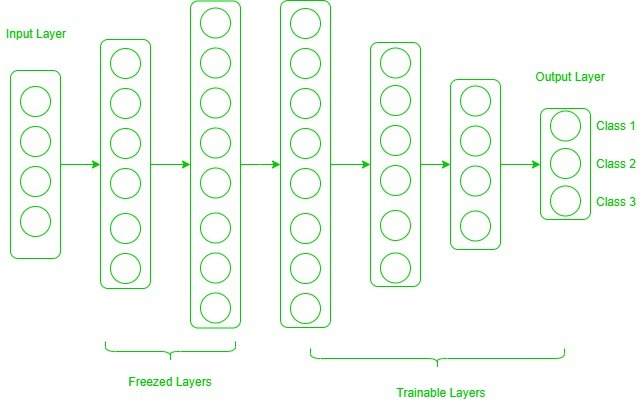
\includegraphics[width=0.7\linewidth]{images/Frozen-layers.jpg}
    \caption{Figure taken from \cite{geeks-transfer-learning} illustrating frozen and trainable layers from pre-trained and fine-tuned network.}
    \label{fig:frozen-layers}
\end{figure}

\subsection{Recommendations}

\begin{itemize}
    \item \textbf{The target dataset is small and similar to the base network dataset}: There may be an issue of overfitting because fine-tune the pre-trained network with the target dataset may not generalise to the global population. Also, there may be some changes in the number of classes in the target task; remove the fully connected layers from the end and add a new fully connected layer satisfying the number of new classes. Now, we freeze the rest of the model and only train newly added layers \cite{geeks-transfer-learning}.
    \item \textbf{The target dataset is small and different from the base network dataset}: Since the target dataset is different, using high-level features of the pre-trained model will not be useful. In such a case, remove most of the layers from the end in a pre-trained model, and add new layers a satisfying number of classes in a new dataset. This way we can use low-level features from the pre-trained model and train the rest of the layers to fit a new dataset. Sometimes, it is beneficial to train the entire network after adding a new layer at the end \cite{geeks-transfer-learning}.
    \item \textbf{Set the learning rate to be low}: It is essential to utilize a lower learning rate when compiling the new model because you are training a much larger model and want to readjust the pretrained weights. If not, your model may rapidly become overfit \cite{geeks-transfer-learning}.
\end{itemize}

\printbibliography

\end{document}